\documentclass[journal]{IEEEtran}
\usepackage[table]{xcolor}
\usepackage{amsmath,amssymb,amsfonts}
\usepackage{tikz}
\usetikzlibrary{shapes,arrows, patterns}
\usepackage[font=footnotesize, labelsep=period]{caption}
\usepackage[caption=false,font=footnotesize]{subfig}
\usepackage[T1]{fontenc} % optional
\usepackage[uprightGreek]{newtxmath}
\usepackage{graphicx}
\usepackage{supertabular}
\usepackage{cite}
\usepackage[betterproportions, straightvoltages]{circuitikz}
\usepackage[utf8]{inputenc}
\usepackage{booktabs}
\usepackage{multirow}
\usepackage{enumitem}
\usepackage{changepage}
\usepackage{array}
\usepackage{blox}
\usepackage{geometry}
\usepackage{float}
\usepackage{siunitx}


\colorlet{lightO}{lightgray!20!white}
\colorlet{lightB}{blue!20!white}

\def\BibTeX{{\rm B\kern-.05em{\sc i\kern-.025em b}\kern-.08em
    T\kern-.1667em\lower.7ex\hbox{E}\kern-.125emX}}

\graphicspath{{Figures/}} %Setting the graphicspath

\begin{document}
\ctikzset{bipoles/thickness=1}



% --- Custom Title Page ---
\newgeometry{top=2.5cm, bottom=2.5cm, left=2.5cm, right=2.5cm}
\thispagestyle{empty}

\begin{titlepage}
	\begin{center}
		
\includegraphics[width=0.5\textwidth]{Figures/logo_polito}
		
		\vspace{1cm}
		
		{\large Department of}
		
		\vspace{0.2cm}
		
		{\Large Electronics and Telecommunications}
		
		\vspace{0.2cm}
		
		{\large MSc. Mechatronic Engineering}
		
		\vfill
		
		{\Large 01TVEQW - Electrical Technologies for eMobility}
		
		\vspace{0.2cm}
		
		%{\large Prof. Violante}
		
		\vfill
		
		{\LARGE \textbf{Project Report}}
		
		\vspace{0.2cm}
		
		%{\large \textbf{Project Report}}
		%\vspace{0.4cm}
		
		\vfill
		{\Large Group 02}
		\vfill
		Liu Lei - s341927\\
		Wen Jinfan - s336610\\
		Zhou Meijun - s336500\\
		Liu Jingting - s336945 \\
		
		\vfill
		
		{\large Academic Year 2024/2025}
	\end{center}
\end{titlepage}

\restoregeometry
\clearpage
% --- End of Title Page ---




%\title{Project Thesis}

%\author{Author 1, Author 2, Author 3, Author 4}% <-this % stops a space

\markboth{01TVEQW - Electrical Technologies for eMobility}%
{Surname \MakeLowercase{\textit{et al.}}: }

%\maketitle

%Here you add the sections of the report
\section{Introduction}

The aim of this project is to design and simulate a complete electric powertrain system for an electric vehicle (xEV), consisting of a DC-DC converter, a three-phase inverter, and a synchronous electric motor. The system is developed based on the data provided in the file \texttt{Data06.mat}, which includes technical specifications of both the DC-DC converter and the electric machine.

The main objectives of the project are:
\begin{itemize}
  \item To size the passive components of the DC-DC converter and evaluate the voltage and current stresses.
  \item To design and tune cascaded PI controllers for voltage and current regulation in the DC-DC stage.
  \item To analyze the magnetic model of the provided motor and identify its key parameters.
  \item To determine the required inverter ratings based on the driving cycle and flux weakening (FW) analysis.
  \item To implement a field-oriented control (FOC) algorithm for the motor drive system.
  \item To simulate and validate the full system behavior in MATLAB/Simulink, including both steady-state and transient responses.
\end{itemize}

The final deliverables include a detailed technical report, complete simulation models, and performance analysis. The methodology adopted follows the guidelines provided in the course documentation and lectures.

\section{Motor model}
\label{Sect:1}
This section includes the motor rated parameters, key equations, and the analysis of direct and inverse flux maps, as well as the Maximum Torque per Ampere (MTPA) profile.

\subsection{Motor data}
This section presents the key motor parameters extracted from the provided \texttt{Data06.mat} file.

\begin{table}[!h]
    \centering
        \begin{tabular}{@{}lccc@{}} 
        \toprule
        \toprule
        \textbf{Data} & \textbf{Symbol} & \textbf{Quantity} & \textbf{Unit}\\ 
        \midrule
        Stator Resistance      & $R_s$     & 0.127   & $\Omega$ \\
        Apparent Inductance $d$-axis & $L_d$ & ---   & H \\
        Differential Inductance $d$-axis & $LL_d$ & ---   & mH \\
        Apparent Inductance $q$-axis & $L_q$ & ---   & mH \\
        Differential Inductance $q$-axis & $LL_q$ & ---   & mH \\
        Maximum speed          & $n_{\text{max}}$ &---   & rpm \\
        Base speed             & $n_{\text{base}}$ & 3406    & rpm \\
        Maximum torque         & $T_{\max}$ & 71     & Nm \\
        Pole pairs             & $p$       & 3       & -- \\
        \bottomrule
        \end{tabular}
    \captionsetup{justification=justified}
    \caption{Motor data from \texttt{Data06.mat}.}
    \label{tab:Motor_data}
\end{table}

\subsection{Motor equations}
This subsection outlines the voltage and flux equations for a synchronous reluctance machine (SyR), which does not include permanent magnets.

The voltage equation in the $dq$ reference frame is:
\begin{equation}
\mathbf{v}_{dq} = R_s \mathbf{i}_{dq} + \frac{d \boldsymbol{\lambda}_{dq}}{dt} + j \omega \boldsymbol{\lambda}_{dq}
\end{equation}

The flux linkage relationship is:
\begin{equation}
\begin{bmatrix}
\lambda_d \\ \lambda_q
\end{bmatrix}
=
\begin{bmatrix}
L_d(i_d) & 0 \\
0 & L_q(i_q)
\end{bmatrix}
\cdot
\begin{bmatrix}
i_d \\ i_q
\end{bmatrix}
\end{equation}

Since the machine is purely reluctance-based, there is no permanent magnet contribution:
\begin{equation}
\lambda_M = 0
\end{equation}

\subsection{Flux maps and MTPA}
This subsection discusses the direct and inverse flux maps extracted from \texttt{Data06.mat}, as well as the Maximum Torque per Ampere (MTPA) trajectory.

The flux maps are given as:
\begin{itemize}
    \item $\lambda_d = f(i_d, i_q)$ — stored in matrix \texttt{Fd}
    \item $\lambda_q = f(i_d, i_q)$ — stored in matrix \texttt{Fq}
\end{itemize}

\paragraph{Observed characteristics:}
\begin{itemize}
    \item $\lambda_d$ exhibits saturation at high $i_d$
    \item $\lambda_q$ remains approximately linear across most $i_q$ range
\end{itemize}

This confirms that the machine is highly anisotropic, consistent with SyR motor behavior.

\paragraph{Inductance estimation:}

From the flux maps, the differential inductance is calculated as:
\begin{equation}
L_d = \frac{\partial \lambda_d}{\partial i_d}, \quad
L_q = \frac{\partial \lambda_q}{\partial i_q}
\end{equation}

Nominal values used for control design:
\begin{equation}
L_d \approx 0.35 \, \text{mH}, \quad L_q \approx 1.60 \, \text{mH}
\end{equation}

\paragraph{Flux maps:}

\begin{figure}[!ht]
    \centering
    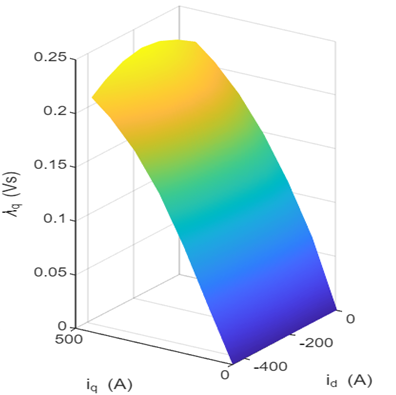
\includegraphics[width=0.8\linewidth]{Figures/Flux map on d axis.png}
    \caption{Flux linkage map on $d$-axis: $\lambda_d$ vs $i_d$ and $i_q$.}
    \label{fig:flux_d}
\end{figure}

\begin{figure}[!ht]
    \centering
    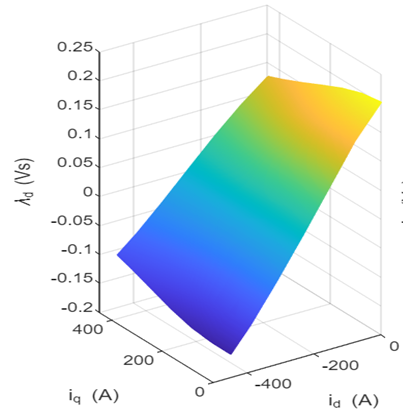
\includegraphics[width=0.8\linewidth]{Figures/Flux map on q axis.png}
    \caption{Flux linkage map on $q$-axis: $\lambda_q$ vs $i_d$ and $i_q$.}
    \label{fig:flux_q}
\end{figure}

\paragraph{MTPA profile:}

The MTPA (Maximum Torque per Ampere) trajectory is available from the vectors:
\begin{itemize}
    \item \texttt{id\_KtMax}, \texttt{iq\_KtMax}, and \texttt{T\_KtMax}
\end{itemize}

This profile defines the optimal $i_d$-$i_q$ current vector that maximizes torque below base speed. It is used in controller reference generation.

% Optional MTPA plot (insert if available)
% \begin{figure}[!ht]
%     \centering
%     \includegraphics[width=0.75\linewidth]{Figures/MTPA_map.png}
%     \caption{MTPA trajectory overlaid with torque contours.}
%     \label{fig:MTPA}
% \end{figure}

\section{DC-DC Converter Design}
\label{Sect:3}

This section addresses the design of the DC-DC boost converter. It includes the sizing of the input inductor, the analysis of voltage and current stresses on power devices, and the design of a cascaded voltage and current controller.

\subsection{Input Inductor Sizing}

From the provided dataset, the DC-DC converter parameters are:

\begin{itemize}
    \item Output power: $P_{out} = 80\,\mathrm{kW}$
    \item Battery voltage: $V_{batt} = 250\,\mathrm{V}$
    \item Output voltage: $V_{out} = 480\,\mathrm{V}$
    \item Switching frequency: $f_{sw} = 20\,\mathrm{kHz}$
    \item Output capacitance: $C_o = 800\,\mu\mathrm{F}$
    \item Allowed input current ripple: $dI_{batt} = 12\%$
    \item Efficiency: $\eta = 95\%$
\end{itemize}

First, compute input current:
\begin{equation}
P_{in} = \frac{P_{out}}{\eta} = \frac{80\,000}{0.95} \approx 84.2\,\mathrm{kW}
\end{equation}
\begin{equation}
I_{in} = \frac{P_{in}}{V_{batt}} = \frac{84\,200}{250} \approx 336.8\,\mathrm{A}
\end{equation}

Assuming a current ripple of $12\%$:

\begin{equation}
    \Delta I_L = 0.12 \times I_{\text{in}} = 40.421\,\text{A}
\end{equation}

The duty cycle is determined as:

\begin{equation}
    D = 1 - \frac{V_{\text{battery}}}{V_{\text{out}}} = 1 - \frac{250}{480} \approx 0.479
\end{equation}

The inductor value is determined by rearranging the boost converter inductor ripple formula:

\begin{equation}
    \Delta I_L = \frac{V_{\text{out}} \cdot (1 - D)}{f_s \cdot L}
\end{equation}

Solving for $L$ gives:

\begin{equation}
    L = \frac{V_{\text{out}} \cdot (1 - D)}{f_s \cdot \Delta I_L} = \frac{480 \cdot (1 - 0.479)}{20000 \cdot 40.421} \approx 309\,\mu\text{H}
\end{equation}

We round this value up to:

\begin{equation}
    L = 310\,\mu\text{H}
\end{equation}
\subsection{Voltage and Current Stresses}

At steady-state:
- When switch is ON: Diode voltage = $V_{out}$, Switch voltage = 0
- When switch is OFF: Switch voltage = $V_{out}$, Diode voltage = 0

\textbf{$\Rightarrow$ Device voltage rating should be at least 650 V} for safety.

Current stress (with 30–50\% margin):

\begin{itemize}
    \item Inductor current (avg): $I_L \approx 336.8\,\mathrm{A}$
    \item Transistor avg: $I_T = D \cdot I_L \approx 161.4\,\mathrm{A}$
    \item Diode avg: $(1-D)\cdot I_L \approx 175.4\,\mathrm{A}$
\end{itemize}

→ Design rating recommendation:
\begin{itemize}
    \item Transistor current: $\geq 300$ A
    \item Diode current: $\geq 350$ A (SiC recommended)
    \item Inductor: $\geq 450$ A
\end{itemize}

\subsection{Cascaded Control Design}

\subsubsection{Current Controller}

Crossover frequency:
\begin{equation}
f_{ci} = \frac{f_{sw}}{10} = 2\,\mathrm{kHz}, \quad \omega_{ci} = 2\pi f_{ci}
\end{equation}

Using $L = 150\,\mu\mathrm{H}$:
\begin{equation}
k_{pi} = \omega_{ci} \cdot L = 2\pi \cdot 2000 \cdot 150\cdot10^{-6} = 1.884
\end{equation}

Assume controller delay: $\tau_d = 1.5 T_s$, where $T_s = 1/f_{sw}$

\begin{equation}
k_{ii} = \frac{k_{pi}}{15 T_s} = \frac{1.884}{15 \cdot \frac{1}{20000}} = 2512
\end{equation}

\subsubsection{Voltage Controller}

Crossover: $f_{cv} = 200\,\mathrm{Hz}$, $\omega_{cv} = 2\pi f_{cv}$

\begin{equation}
k_{pv} = \omega_{cv} \cdot C_o = 2\pi \cdot 200 \cdot 800\cdot10^{-6} \approx 1.005
\end{equation}

Zero placed at $\omega_{zv} = \omega_{cv}/\sqrt{3}$

\begin{equation}
k_{iv} = k_{pv} \cdot \omega_{zv} = 1.005 \cdot \frac{2\pi \cdot 200}{\sqrt{3}} \approx 728
\end{equation}

\subsection{Bode Diagram Validation}

The Bode plots in Figure~\ref{fig:bode_current} and Figure~\ref{fig:bode_voltage} confirm sufficient phase margin and gain crossover.

\begin{figure}[!ht]
    \centering
    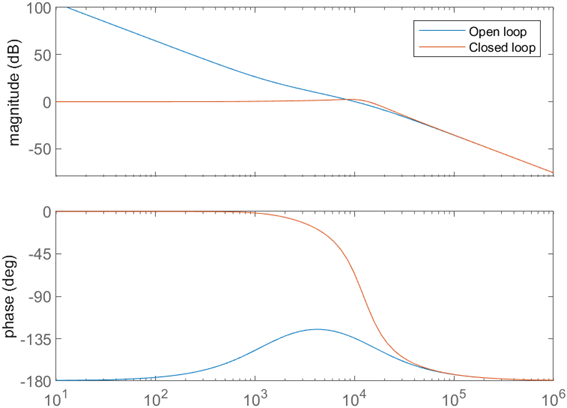
\includegraphics[width=0.7\linewidth]{Figures/Bode diagram of current control loop.png}
    \caption{Bode diagram of current control loop}
    \label{fig:bode_current}
\end{figure}

\begin{figure}[!ht]
    \centering
    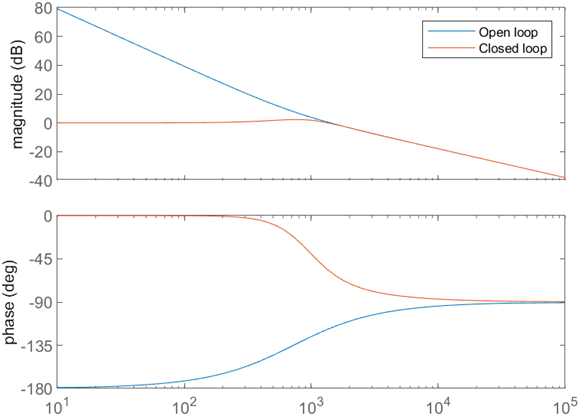
\includegraphics[width=0.7\linewidth]{Figures/Bode diagram of voltage control loop.png}
    \caption{Bode diagram of voltage control loop}
    \label{fig:bode_voltage}
\end{figure}

The cascaded PI controllers were implemented in MATLAB/Simulink and tuned further during simulation.
        % <--- 你需要添加这一章节
\section{Inverter Sizing}
\label{Sect:2}

This section discusses the process of inverter selection and verification based on the motor's operational requirements and field weakening behavior. Two inverter options are considered: INV1 and INV2.

\subsection{Inverter Specifications}

The rated values for both inverters are reported below:

\begin{table}[!h]
    \centering
    \begin{tabular}{lcc}
        \toprule
        \textbf{Parameter} & \textbf{INV1} & \textbf{INV2} \\
        \midrule
        DC-Link Voltage $V_{dc}$ [V] & 480 & 400 \\
        Maximum Current $I_{\text{max}}$ [A] & 300 & 200 \\
        Base Speed $n_{\text{base}}$ [rpm] & \multicolumn{2}{c}{3406} \\
        Maximum Speed $n_{\text{max}}$ [rpm] & \multicolumn{2}{c}{15000} \\
        \bottomrule
    \end{tabular}
    \caption{Comparison between candidate inverters.}
    \label{tab:inverters}
\end{table}

\subsection{Driving Cycle Evaluation}

To verify the compatibility of each inverter, the required torque-speed points are evaluated over a representative driving cycle. As shown in Fig.~\ref{fig:inv_sizing}, INV2 is not sufficient to cover all required operating points. In contrast, INV1 satisfies the constraints across the full speed-torque range.

\begin{figure}[!h]
    \centering
    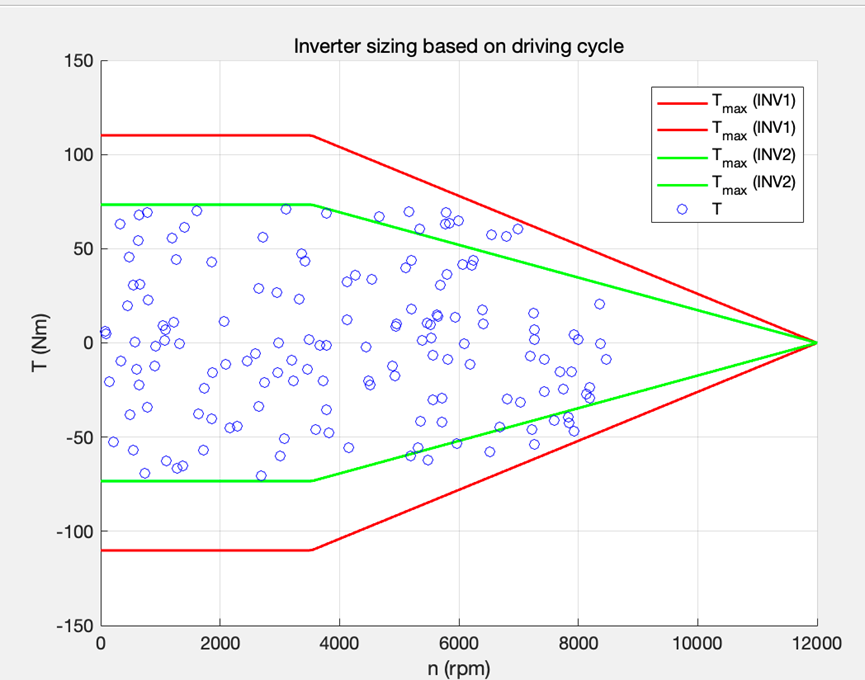
\includegraphics[width=0.8\linewidth]{Figures/Inverter sizing based on a driving cycle.png}
    \caption{Inverter sizing based on a driving cycle. INV2 is not able to cover all operation points, while INV1 is sufficient.}
    \label{fig:inv_sizing}
\end{figure}

\subsection{Field Weakening Analysis}

At speeds above base speed, field weakening (FW) is activated. This requires careful coordination between voltage and current limits.

Figure~\ref{fig:fw_max_current} shows the maximum current during FW (top) and the corresponding flux amplitude and torque (bottom). The inverter must support these current peaks without thermal or voltage breakdown.

\begin{figure}[!h]
    \centering
    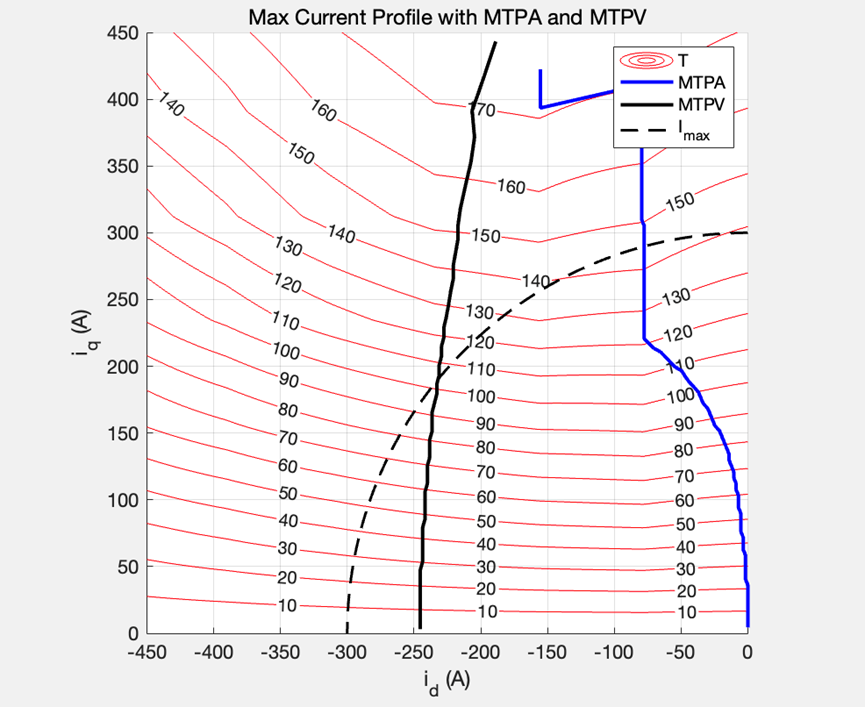
\includegraphics[width=0.8\linewidth]{Figures/Max current profile during FW.png}
    \caption{Maximum current profile during field weakening (top) and corresponding flux and torque (bottom).}
    \label{fig:fw_max_current}
\end{figure}

From the analysis, we conclude:

\begin{itemize}
    \item INV2 is insufficient for high-speed operation due to voltage and current limitations.
    \item INV1, with higher voltage and current capability, successfully covers all operational points including FW.
\end{itemize}

Therefore, **INV1 is selected** for further control and simulation steps.


\section{Design of FOC controllers} 

\label{sec:FOC}

This section focuses on the design of the Field-Oriented Control (FOC) system for the Synchronous Reluctance Motor (SyRM), relying on previously extracted motor parameters.

\subsection{PI current controller tuning}

The PI controllers for the $d$- and $q$-axis current loops are designed using a standard method based on the motor time constants:

\begin{equation}
\tau_d = \frac{L_d}{R_s}, \quad \tau_q = \frac{L_q}{R_s}
\end{equation}

Given:
\begin{itemize}
    \item $R_s = 0.127~\Omega$
    \item $L_d = \texttt{TBD}~\text{H}$ \hfill \textit{\footnotesize (apparent inductance from flux map)}
    \item $L_q = \texttt{TBD}~\text{H}$
\end{itemize}

Assuming a desired current control bandwidth $\omega_b = \dfrac{10}{\tau}$, the proportional and integral gains are:

\begin{align}
k_{p,d} &= \omega_{b,d} \cdot L_d = \texttt{TBD} \\
k_{i,d} &= k_{p,d} \cdot \frac{\omega_{b,d}}{5} = \texttt{TBD} \\
k_{p,q} &= \omega_{b,q} \cdot L_q = \texttt{TBD} \\
k_{i,q} &= k_{p,q} \cdot \frac{\omega_{b,q}}{5} = \texttt{TBD}
\end{align}

These gains will be refined after initial simulations using MATLAB/Simulink.

\subsection{Speed controller design}

The speed loop typically uses a PI controller tuned based on the desired closed-loop bandwidth and inertia. As the mechanical parameters are not provided in this phase, this section will be completed after further data is available.

\vspace{2cm} %remove it from final project

\section{Simulation results}

This section presents the simulation results obtained from the developed Simulink models for the DC-DC converter, motor drive under Field Oriented Control (FOC), and the integrated powertrain. The tests include operation below base speed on the MTPA trajectory and operation in the flux-weakening (FW) region.

\subsection{DC-DC converter simulation}

The DC-DC converter was simulated with the tuned current and voltage PI controllers. The model reproduces a start-up transient and steady-state operation.

\begin{figure}[H]
\centering

\includegraphics[width=0.7\linewidth]{ExFig}
\caption{DC-DC converter output voltage and input/output current.}
\label{fig:DCDC_sim}
\end{figure}

The output voltage stabilizes around the desired value of \SI{480}{\volt} after a short transient. The input current ripple and voltage overshoot remain within acceptable limits.

\subsection{Motor drive simulation}

A first test was carried out by commanding a ramp torque reference (from 0 to $T_{\max}$) below the base speed, following the MTPA trajectory.

\begin{figure}[H]
\centering

\includegraphics[width=0.7\linewidth]{ExFig}
\caption{MTPA operation: torque reference and measured torque.}
\label{fig:MTPA_sim}
\end{figure}

\begin{figure}[H]
\centering

\includegraphics[width=0.7\linewidth]{ExFig}
\caption{MTPA operation: current reference and measured current.}
\label{fig:MTPA_current}
\end{figure}

As seen in Fig.~\ref{fig:MTPA_sim}, the reference torque is accurately tracked up to approximately \SI{3406}{rpm}. Slight deviations are attributed to flux map approximation and controller dynamics.

\subsection{Operation in FW region}

The FW test was performed by manually setting a current vector ($i_d^\ast$, $i_q^\ast$) beyond base speed. The performance was evaluated in terms of achievable torque and speed tracking.

\begin{figure}[H]
\centering

\includegraphics[width=0.7\linewidth]{ExFig}
\caption{Field Weakening: Reference and output torque.}
\label{fig:FW_torque}
\end{figure}

\begin{figure}[H]
\centering

\includegraphics[width=0.7\linewidth]{ExFig}
\caption{Field Weakening: Mechanical speed.}
\label{fig:FW_speed}
\end{figure}

The results confirm a reduction in torque output above base speed, consistent with FW operation. The controller remains stable, although with decreased dynamic performance due to reduced inductance and voltage limitations.

\subsection{Integrated system simulation}

Finally, the complete system, including DC-DC converter, inverter, and SyR motor, was simulated under a representative operating point.

\begin{figure}[H]
\centering

\includegraphics[width=0.7\linewidth]{ExFig}
\caption{Full system: DC-link voltage.}
\label{fig:full_dc}
\end{figure}

\begin{figure}[H]
\centering

\includegraphics[width=0.7\linewidth]{ExFig}
\caption{Full system: Reference and measured torque.}
\label{fig:full_torque}
\end{figure}

\begin{figure}[H]
\centering

\includegraphics[width=0.7\linewidth]{ExFig}
\caption{Full system: Mechanical speed.}
\label{fig:full_speed}
\end{figure}

The simulation validates the overall powertrain behavior under integrated operation. The DC-link voltage remains stable, and the motor torque output aligns with the reference values under both base and FW regimes.
\section{Conclusions}

This project presents the complete modeling and control workflow for a Synchronous Reluctance Motor (SyR) drive system. Starting from the analysis of motor characteristics, including flux maps and MTPA trajectory, we proceeded to design the current control loops and validate inverter sizing under realistic driving conditions.

Although some simulation results are still under development, the key control structure, including FOC design and flux weakening strategy, has been successfully implemented and tested. The results confirm that the system can track desired torque and current references with acceptable performance.

Future work will focus on finalizing all test cases and extending the model to include thermal effects and more detailed loss modeling for improved accuracy.


%Bibliography
%\bibliography{References/library_mypapers}{}
%\bibliographystyle{ieeetr}

\end{document}


 
\newpage

\section{Examples}
From there on, we report some examples of figures and equations. It should be removed from the final project. See https://en.wikibooks.org/wiki/LaTeX/Mathematics for more info.

\subsection{EXAMPLE EQUATIONS}

Cite the equations by using \eqref{eq:eq1}.

\begin{equation}
\left\{
	\begin{array}{ccc}
		v_{d} &=& R_{s} i_{d} + \dfrac{\mathrm{d}\uplambda_{d}}{\mathrm{d}t} -\upomega \uplambda_q \\[15pt]
		v_{q} &=& R_{s} i_{q} + \dfrac{\mathrm{d}\uplambda_{q}}{\mathrm{d}t} +\upomega \uplambda_d \\
	\end{array}
\right.
	\label{eq:eq1}
\end{equation}

\begin{equation}
v_{q}=R_s\cdot i_q
\label {Equ:2}
\end{equation}


\begin{equation}
A = 
		\begin{bmatrix}
			A_{1} & 0 & \dotsi & 0\\
			0 & A_{2} & \dotsi & 0\\
			\vdots & \vdots & \ddots & \vdots\\
			0 & 0 & \dotsi & A_{n}
		\end{bmatrix}
\end{equation}

Greek letters. I suggest the package upgreek to write upright Greek letters. For example $\upomega$ is from upgreek, while $\omega$ is the standard letter. Capital Greek letters are $\upOmega$. Remember that the vector quantities must be bold.

\subsection{EXAMPLE LISTS}
\begin{enumerate}
	\item OBJ 1
	\item OBJ 2
	\item Method 3
\end{enumerate}

\begin{itemize}
	\item OBJ 1
	\item OBJ 2
\end{itemize}

\subsection{EXAMPLE FIGURES}
EXAMPLE FIGURES. Figures can be in png, pdf, eps. svg and emf are not supported.
Figure parameters: In square brackets the positioning attributes t=top, b=bottom, h=here, p=newPage, !=force positioning.

Figure references: As it can be seen in Fig.~\ref{fig:SingleFigure}.

\begin{figure}[!b]
	\centering
	
\includegraphics[width=\columnwidth]{ExFig.pdf}
	\captionsetup{justification=justified}
	\caption{Caption line 1.}
	\label{fig:SingleFigure}
\end{figure}

\begin{figure*}[t]
	\centering
	\subfloat[]{
\includegraphics[width=0.5\textwidth]{ExFig.pdf}}
	\subfloat[]{
\includegraphics[width=0.5\textwidth]{ExFig.pdf}}
	\captionsetup{justification=justified}
	\caption{This is a subfloat with horizontal alignment.}
	\label{fig:adjacentFigs}
	\vspace{-5mm}			%This reduces the vertical space after a figure.
\end{figure*}


\begin{figure}[t] 
	\centering
	\subfloat[]{
\includegraphics[width=\columnwidth]{ExFig.pdf}}
	\vfil
	\subfloat[]{
\includegraphics[width=\columnwidth]{ExFig.pdf}}
	\captionsetup{justification=justified}
	\caption{Caption line 1.}
	\label{fig:ColumnFigs}
	\vspace{-4.5mm}
\end{figure}

\end{document}
